\section{Network architecture}
Using all the concept described in the previous sections it is possible to describe the plant monitoring system application. All the following steps has been made by using the guide developed by Laurent Deru, Sébastien Dawans and Mathieu Ocana, available in GitHub under permissive 3-clause BSD-style open source license. However, in the tutorial it is used only TelosB node instead of the Texas Instrument Sensor Tags that is used in this development of a plant monitoring system.\\
\begin{figure}[!h]
	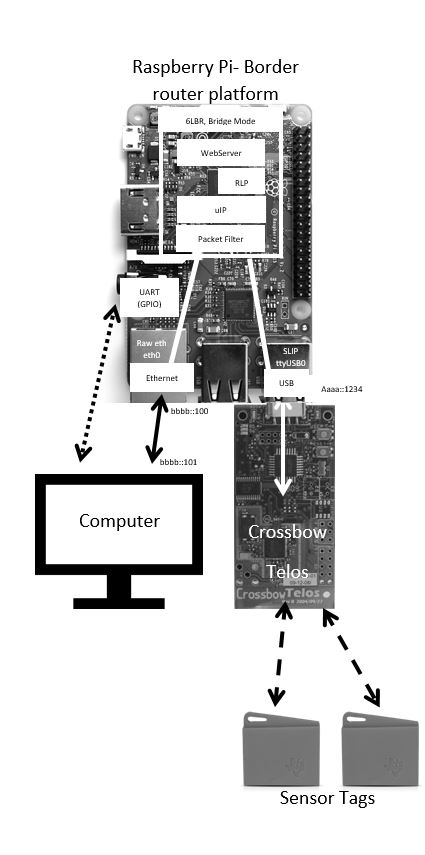
\includegraphics[width=\linewidth]{Network}
	\caption{Development of the network}
	\label{fig:Network}
\end{figure}
\subsection{The network}
The network main idea is well depicted in fig\ref{fig:Network}. The raspberry pi act as a six low pan border router (6LBR) and act as a link between the Ethernet and the wireless sensor network. The wireless sensor network is composed by the TelosB that act as a sink for all the other sensor tags. The TelosB sensor is attached via USB to the Raspberry Pi.
On the other hand, the Raspberry Pi is connected to a computer via a normal house router.\cite{6LBR}
The Raspberry Pi connect the two subnets via RPL protocol on the wireless sensor network side and NPD on the Ethernet part.\cite{mode}\\
\subsection{WebServer}



